\documentclass[tikz]{standalone}

\usetikzlibrary{arrows.meta,calc}

\tikzset{
    pics/anode/.style args={#1,#2,#3}{
        code={
            \path[draw, pic actions] (-4.85mm,-4.85mm) rectangle(4.85mm, 4.85mm);
            \node at (-3mm,-3mm) {\footnotesize #1};%G;
            \node at (3mm,-3mm){\footnotesize #2};%H
            \node at (-3mm,3mm){\footnotesize #3};%F
        }
    },
    pics/anode/.default={0,0,0},
}

\begin{document}
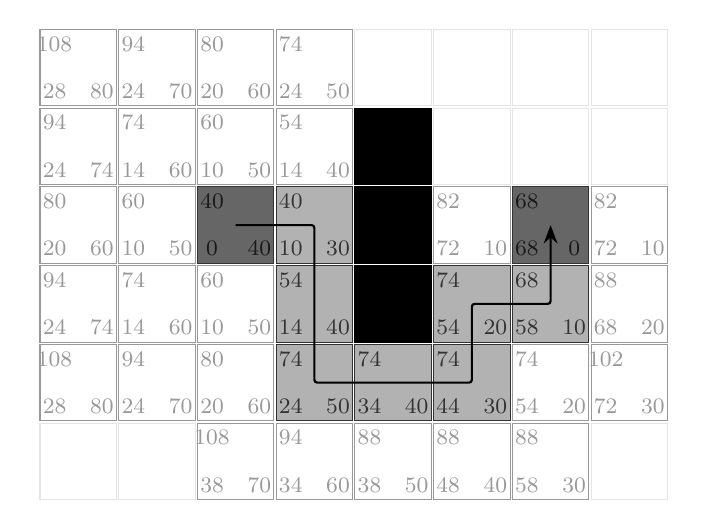
\begin{tikzpicture}[
scaned/.style={draw=black!40, text=black!40},
ending/.style={draw=black!80, fill=black!60, text=black!90},
routed/.style={draw=black!80, fill=gray!60, text=black!80},
]
\node foreach \x in {0,1,...,7} foreach \y in {0,1,...,5} at (\x, \y) [rectangle, draw=gray!20, minimum size=9.7mm] {};
\node foreach \y in {2,3,4} at (4, \y) [rectangle, draw=black, fill=black, minimum size=9.7mm] {};

\pic[scaned] at(0,1) {anode={28,80,108}};
\pic[scaned] at(0,2) {anode={24,74,94}};
\pic[scaned] at(0,3) {anode={20,60,80}};
\pic[scaned] at(0,4) {anode={24,74,94}};
\pic[scaned] at(0,5) {anode={28,80,108}};

\pic[scaned] at(1,1) {anode={24,70,94}};
\pic[scaned] at(1,2) {anode={14,60,74}};
\pic[scaned] at(1,3) {anode={10,50,60}};
\pic[scaned] at(1,4) {anode={14,60,74}};
\pic[scaned] at(1,5) {anode={24,70,94}};

\pic[scaned] at(2,0) {anode={38,70,108}};
\pic[scaned] at(2,1) {anode={20,60,80}};
\pic[scaned] at(2,2) {anode={10,50,60}};
\pic(start)[ending] at(2,3) {anode={0,40,40}};
\pic[scaned] at(2,4) {anode={10,50,60}};
\pic[scaned] at(2,5) {anode={20,60,80}};

\pic[scaned] at(3,0) {anode={34,60,94}};
\pic[routed] at(3,1) {anode={24,50,74}};
\pic[routed] at(3,2) {anode={14,40,54}};
\pic[routed] at(3,3) {anode={10,30,40}};
\pic[scaned] at(3,4) {anode={14,40,54}};
\pic[scaned] at(3,5) {anode={24,50,74}};

\pic[scaned] at(4,0) {anode={38,50,88}};
\pic[routed] at(4,1) {anode={34,40,74}};

\pic[scaned] at(5,0) {anode={48,40,88}};
\pic[routed] at(5,1) {anode={44,30,74}};
\pic[routed] at(5,2) {anode={54,20,74}};
\pic[scaned] at(5,3) {anode={72,10,82}};

\pic[scaned] at(6,0) {anode={58,30,88}};
\pic[scaned] at(6,1) {anode={54,20,74}};
\pic[routed] at(6,2) {anode={58,10,68}};
\pic[ending] at(6,3) {anode={68,0,68}};

\pic[scaned] at(7,1) {anode={72,30,102}};
\pic[scaned] at(7,2) {anode={68,20,88}};
\pic[scaned] at(7,3) {anode={72,10,82}};

\draw[-Stealth,thick,rounded corners=1pt](2,3)-|++(1,-2)-|++(2,1)-|++(1,1);

\end{tikzpicture}
\end{document}
